\section{Silicon Tungsten SiD ECAL}
\begin{figure}
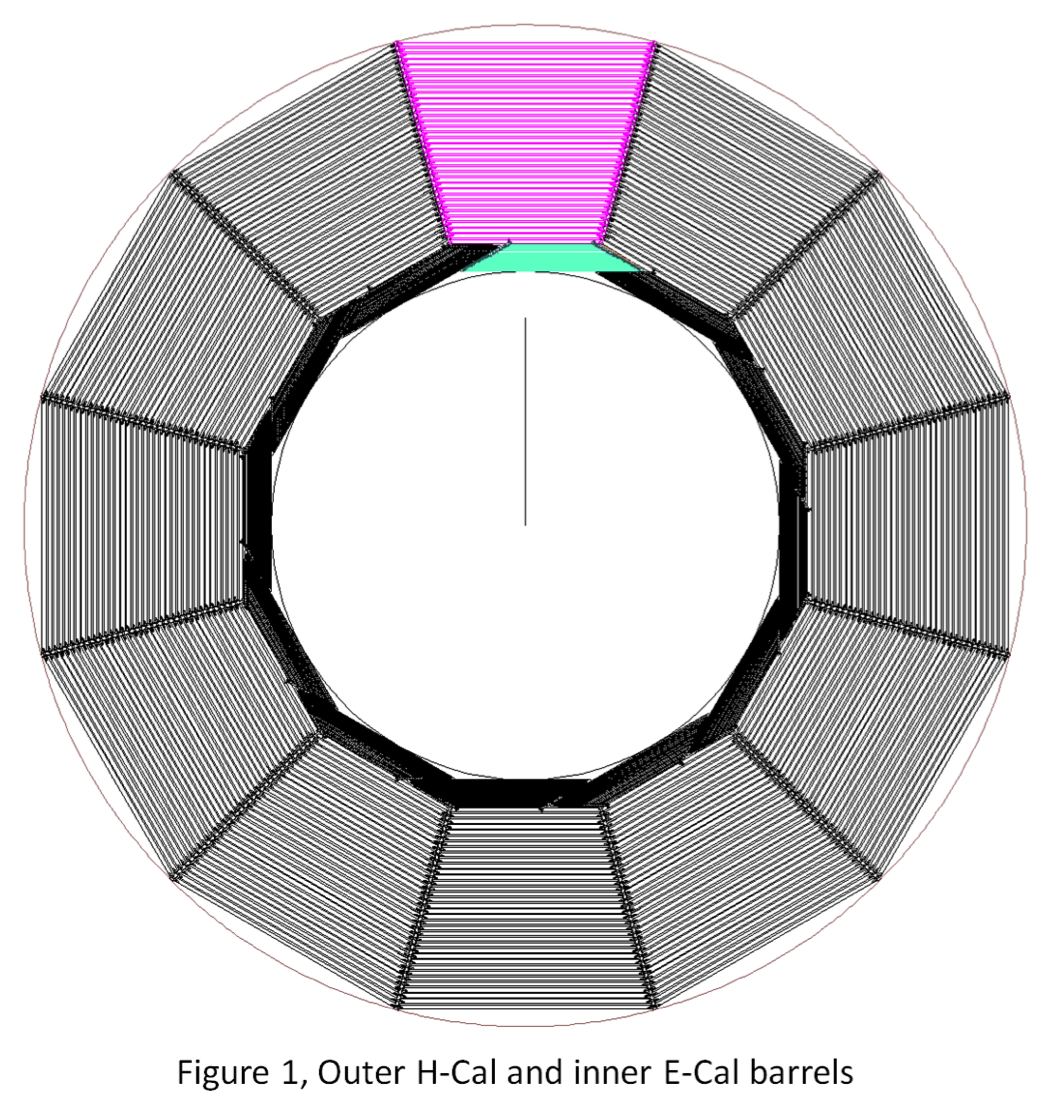
\includegraphics[width=.5\linewidth]{Calorimeter/SiliconTungstenSiD/cross_section}\hfill
\caption{}
\label{fig:Calorimeter:SiDECAL:crosssection}
\end{figure}
\begin{figure}
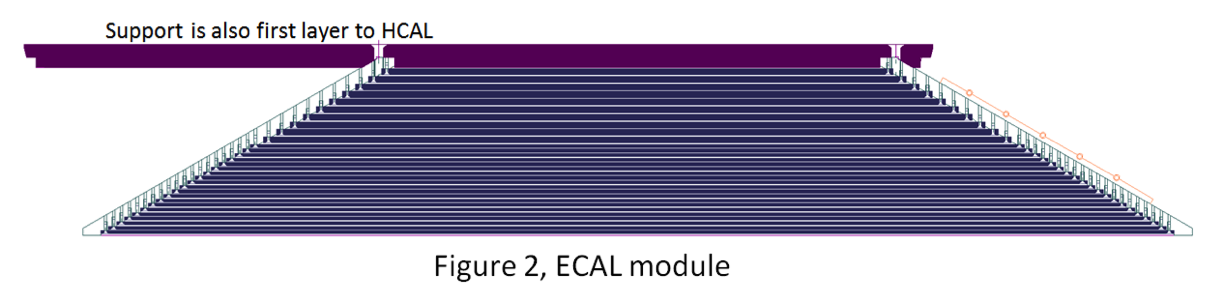
\includegraphics[width=.5\linewidth]{Calorimeter/SiliconTungstenSiD/ecalModule}
\caption{}
\label{fig:Calorimeter:SiDECAL:ecalModule}
\end{figure}
\begin{figure}
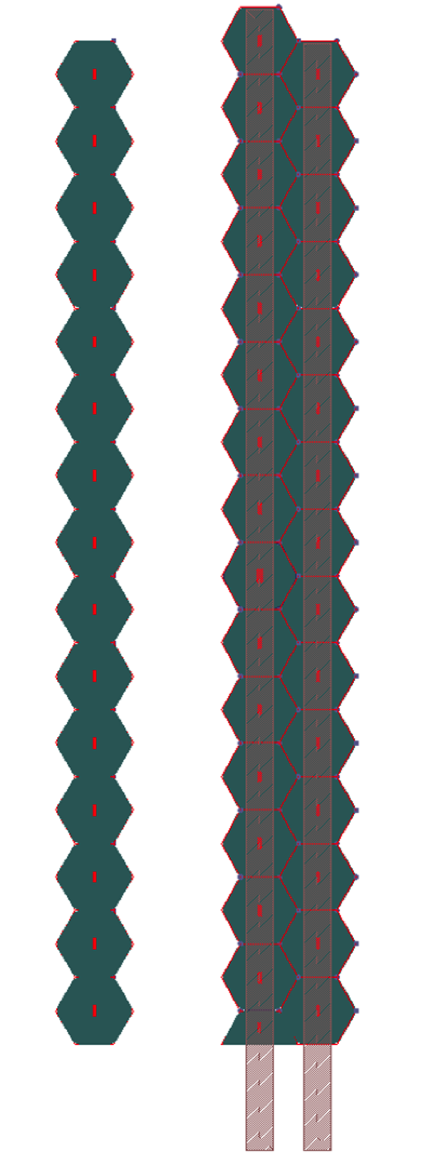
\includegraphics[width=.5\linewidth]{Calorimeter/SiliconTungstenSiD/hexagon} \hfill
\caption{}
\label{fig:Calorimeter:SiDECAL:hexagon}
\end{figure}
\begin{figure}
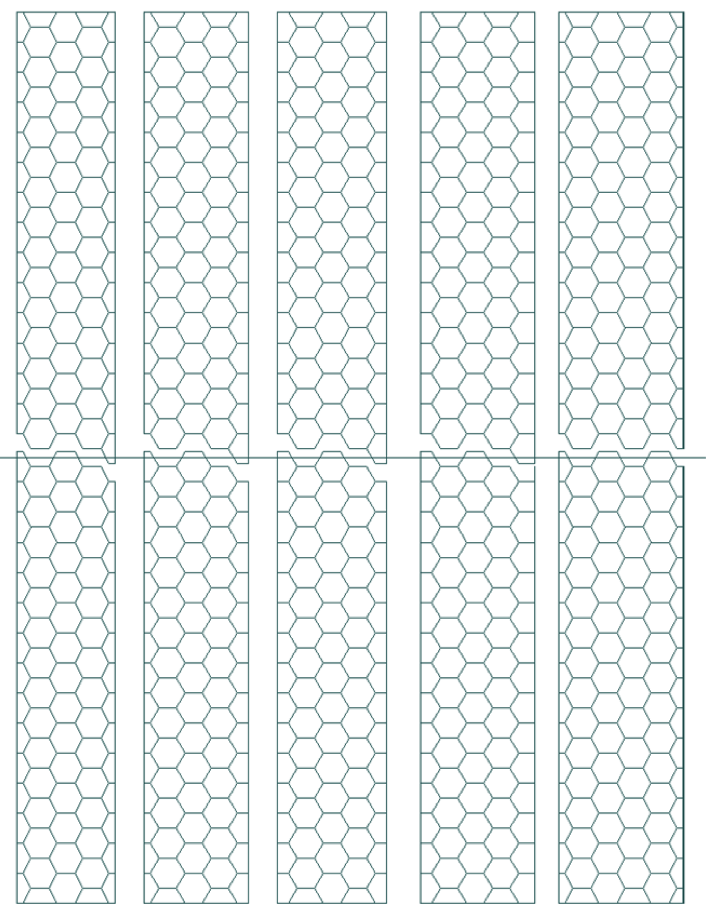
\includegraphics[width=.5\linewidth]{Calorimeter/SiliconTungstenSiD/siliconLayout}
\caption{}
\label{fig:Calorimeter:SiDECAL:siliconLayout}
\end{figure}
\begin{figure}
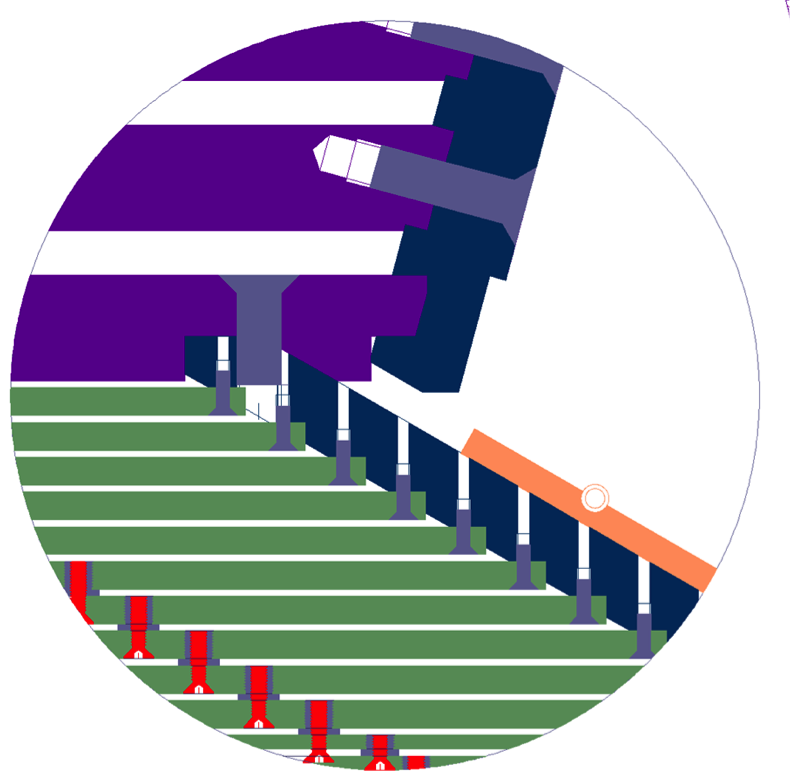
\includegraphics[width=.5\linewidth]{Calorimeter/SiliconTungstenSiD/edgeFasteners} \hfil
\caption{}
\label{fig:Calorimeter:SiDECAL:edgeFasteners}
\end{figure}
\begin{figure}
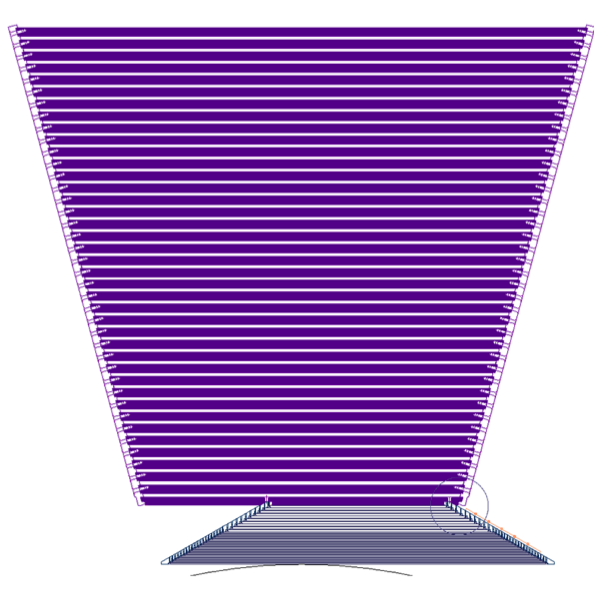
\includegraphics[width=.5\linewidth]{Calorimeter/SiliconTungstenSiD/ecalMounting}
\caption{}
\label{fig:Calorimeter:SiDECAL:ecalMounting}
\end{figure}
\begin{figure}
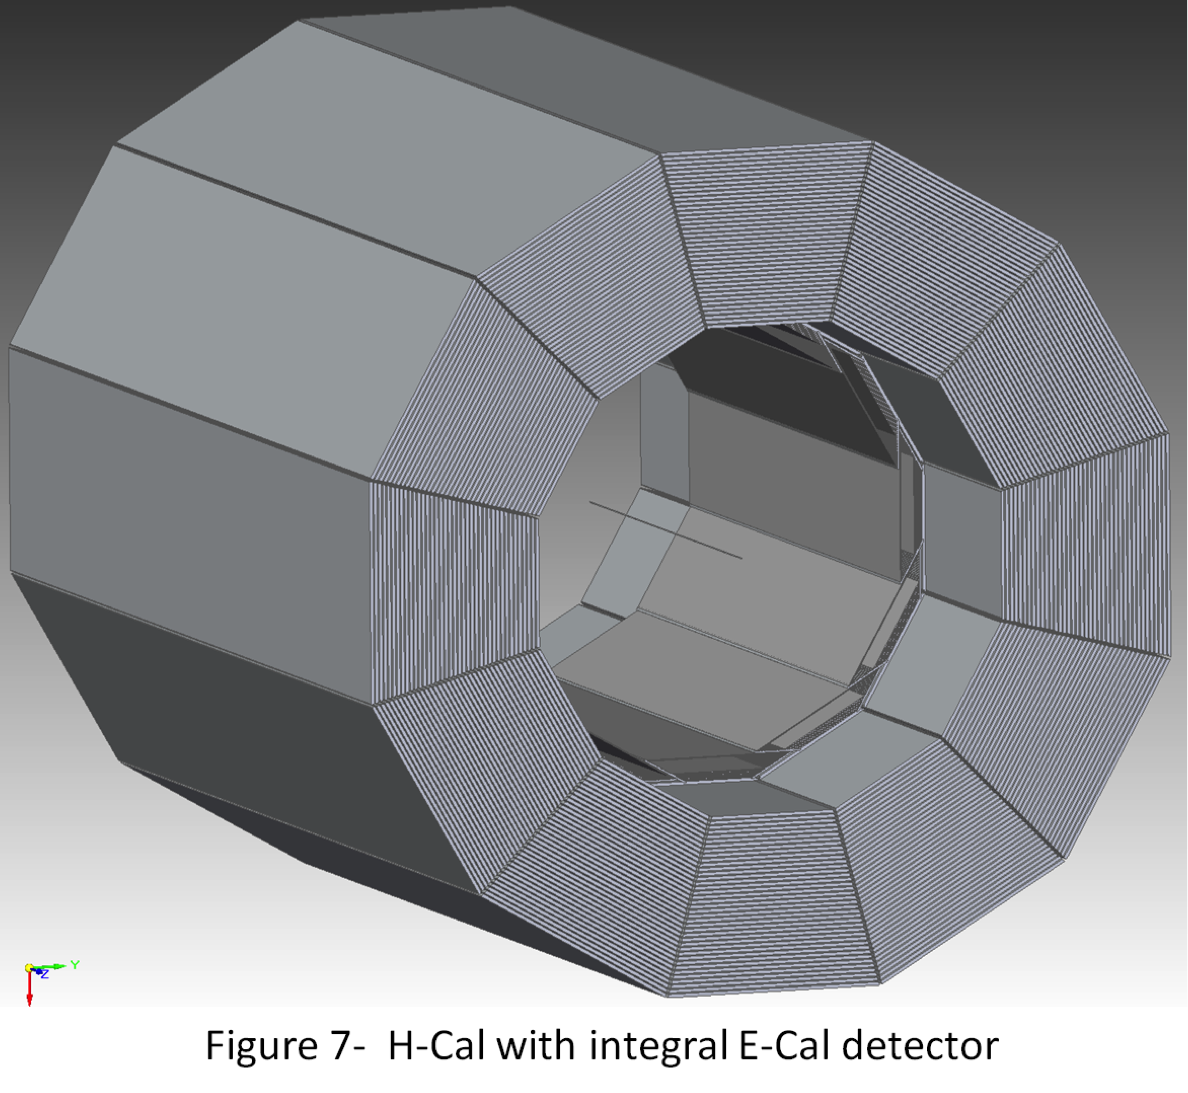
\includegraphics[width=.5\linewidth]{Calorimeter/SiliconTungstenSiD/HCalECal} \hfill
\caption{}
\label{fig:Calorimeter:SiDECAL:HCalECal}
\end{figure}
\begin{figure}
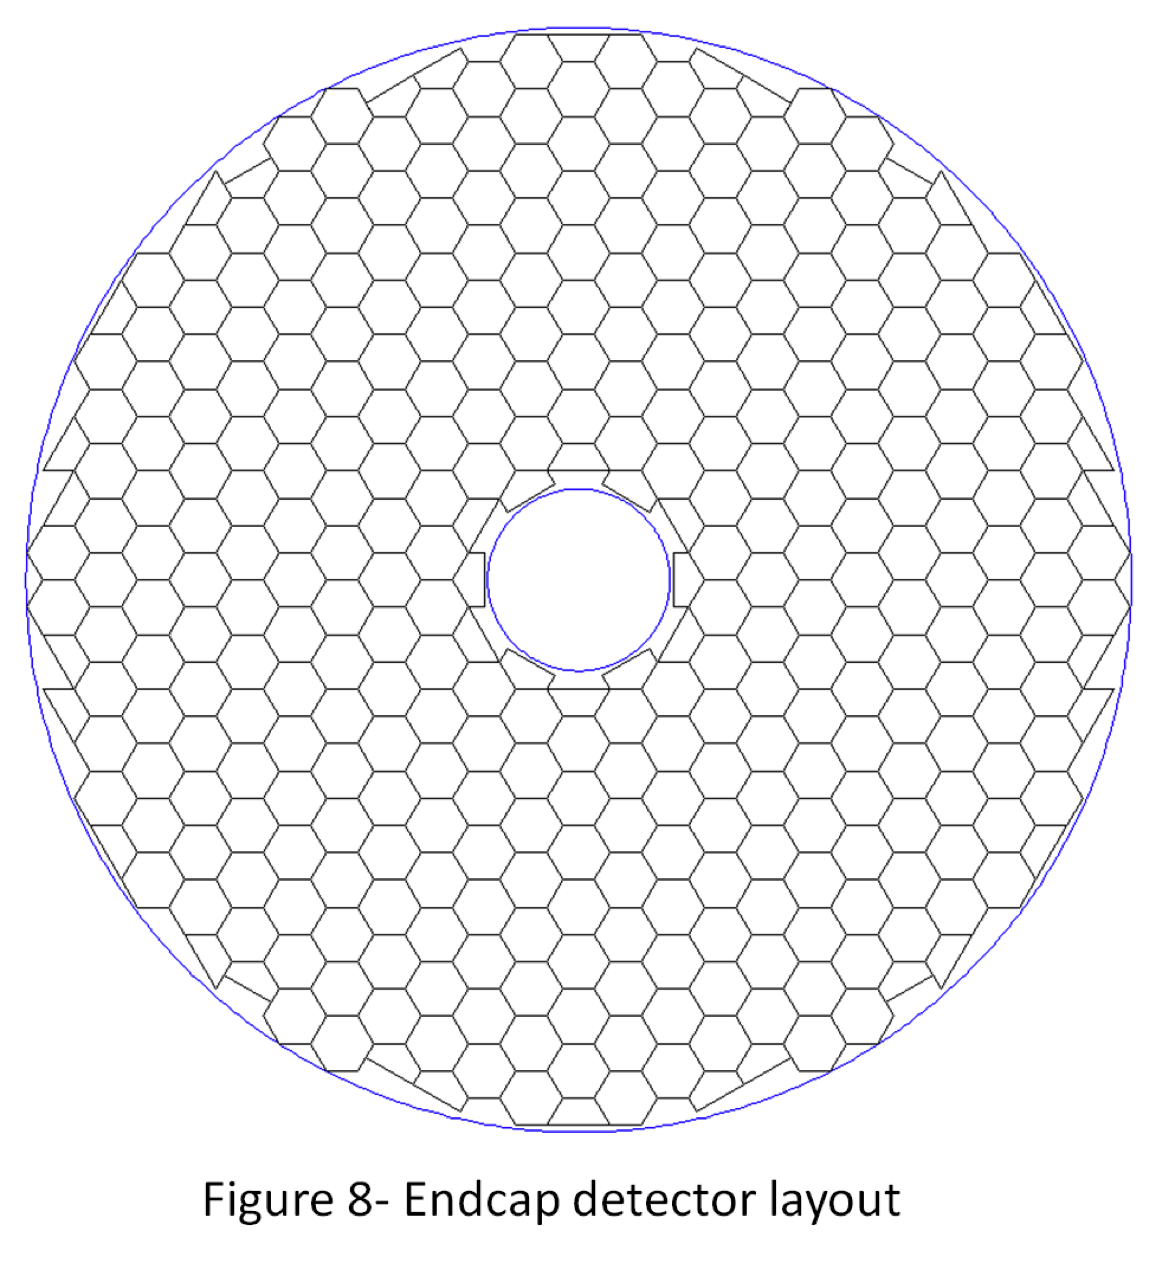
\includegraphics[width=.5\linewidth]{Calorimeter/SiliconTungstenSiD/endcapLayout}
\caption{}
\label{fig:Calorimeter:SiDECAL:endcapLayout}
\end{figure}

This note describes the theory of the mechanical aspects of the E-Cal system for
SiD. The E-Cal barrel consists of stacks of tungsten heavy metal plates which
are arranged in modules surrounding the beamline. Full cylindrical coverage of
the baseline design is attained with twelve modules (see Figure~\ref{fig:Calorimeter:SiDECAL:crosssection}) occupying a
radial envelope from \unit[1265]{mm} to \unit[1409]{mm}. The total barrel length is \unit[3.53]{m}. Each
module uses 20 inner plates which are \unit[2.5]{mm} thick followed by ten \unit[5]{mm} thick
plates. Gaps between adjacent plates are \unit[1.25]{mm} and house the silicon detectors
with their associated cables (see Figure~\ref{fig:Calorimeter:SiDECAL:ecalModule}). These hexagonal silicon detectors
are electrically connected to each other with thin, flexible circuits which are
read out on both ends of a module (see Figure~\ref{fig:Calorimeter:SiDECAL:hexagon}). Panels of detectors increase
in width as they get closer to the beamline. To minimize silicon waste and to
maximize coverage, fractions of hexagons complete the panel edges (see figure
4). By cutting the silicon in strategic locations, only a few different silicon
shapes may be needed to achieve the 31 different panel widths. The tungsten
plates are connected together on their longitudinal edges as well as in the
field of detectors. Space for fasteners in the field is achieved by chamfering
the corners of the hexagonal detectors. The field fasteners hold the plates
together, provide a uniform \unit[1.25]{mm} standoff height, and assist with inter-plate
shear. The fasteners near the edges of the plates close the module profile and
lend torsional rigidity to the structure. An FEA simulation of the proposed
configuration should be done to properly size the fasteners (see Figure~\ref{fig:Calorimeter:SiDECAL:edgeFasteners}).The
modules, which weigh about 5 tons each, are mounted to stainless plates which
are used as the first layer of the next detector system (H-Cal). This first
H-Cal plate is unique in that its two longitudinal edges form a guide system to
locate the E-Cal to the H-Cal system. The H-Cal modules are first bolted
together to form the H-Cal barrel. Interleaving structural side battens maintain
spacing for the H-Cal plates and extend inward to the E-Cal support plates. The
inner ends of these battens act in concert as the female portion of the E-Cal
guide system. The E-Cal modules are slid into place in the inner H-Cal bore.
Extension plates complete the inner H-Cal first layer, since the E-Cal barrel is
shorter. H-Cal detector panels are installed after this structure is complete
(see Figure~\ref{fig:Calorimeter:SiDECAL:HCalECal}). Only simple detector layouts have been done for the E-Cal
endcaps so far. These layouts show that using full and partial hexagons could
yield fairly good coverage with only a few shapes. (see Figure~\ref{fig:Calorimeter:SiDECAL:endcapLayout}).
